This use-case is the implementation of the \emph{voluntary-automatic} scenario
presented in the matrix \autoref{tab:matrix}.

\begin{figure}[htb]
    \centering
    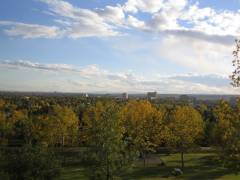
\includegraphics[width=\columnwidth]{Automatic1}
    \caption{Interface of the automatic use-case.}
    \label{fig:Automatic1}
\end{figure}

For the Automatic use case we choose to implement a widely used feature detection
algorithm, the \ac{SIFT}. To perform this load intensive algorithm we used the
power of the \ac{WebCL} framework to greatly speedup the computation.\\

In order to build a working example of the algorithm we started with the creation
of an abstraction layer over the \ac{WebCL} raw implementation, then we created
a small \emph{MultiMedia} library able to compute the needed operation on the
images using our \emph{abstraction layer} eventually we implemented the algorithm
in the \emph{MultiMedia} library.

\paragraph{The abstraction layer} is in charge of the communication with the raw
Nokia WebCL framework as well as creating a stateful object capable of
managing of the I/O data for a WebCL \emph{kernel}.

\paragraph{The MultiMedia library} is used to perform the operation required by
the algorithm (such as \code{blur}, \code{scale}, \code{RGB to gray} etc.) either
using \ac{WebCL} or the built-in HTML5 functions.
\begin{figure}[htb]
    \centering
    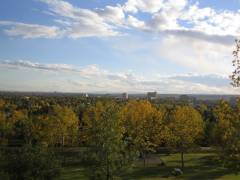
\includegraphics[width=\columnwidth]{Automatic2}
    \caption{Intermediate results of the algorithm.}
    \label{fig:Automatic2}
\end{figure}

\subsection{SIFT alogorithm}
The \ac{SIFT} algorithm is composed of 4 sequential steps: Scale-space extrema
detection, Keypoint localization, Orientation assignment and Keypoint descriptor.

\subsubsection{Scale-space extrema detection}
in this step we generate the so called
scale space representation of the image. In order to do this we need to
convolve the image $I(x,y)$ at different scales $k\sigma$ with a varing
guassian kernel $G(x,y,k\sigma)$ obtainig:
\[
    L(x,y,k\sigma) = G(x,y,k\sigma) \ast I(x,y)
\]
Then the difference of successive blurred images are taken
\[
    D(x,y,\sigma) = L(x,y,k_i\sigma) - L(x,y,k_j\sigma)
\]
This step produce the \ac{DoG} images, the first \emph{Keypoints} are identified
as local minima/maxima of the \ac{DoG} image across scales.



\subsubsection{Keypoint localization}
In this step the \emph{keypoints} are filtered
to remove unstable points and keep only the good ones. This step can be
further subdivided into 3 stages
\begin{itemize}
    \item \emph{Interpolation} of nearby data for accurate position.
    \item \emph{Discarding} low-contrast keypoints.
    \item \emph{Eliminating} edge responses.
\end{itemize}



\subsubsection{Orientation assignment}
In this step for each keypoint is assigned an
orientation and a magnitude. This step is used to achieve \emph{invariance
rotation}. The mangnitude $m(x,y)$ and orientation $\theta(x,y)$ are
calculated as follows:
\begin{equation*}
\begin{split}
    m(x,y)&=\sqrt{\left(L(x+1,y)-L(x-1,y)\right)^2+\left(L(x,y+1)-L(x,y-1)\right)^2}\\
    \theta(x,y)&=\tan^{-1}{\left(\frac{L(x,y+1)-L(x,y-1)}{L(x+1,y)-L(x-1,y)}\right)}
\end{split}
\end{equation*}

\begin{figure}[htb]
    \centering
    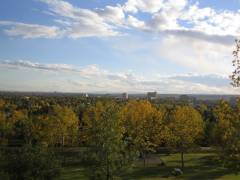
\includegraphics[width=\columnwidth]{Automatic3}
    \caption{\acs{SIFT} result comparison with the reference data.}
    \label{fig:Automatic3}
\end{figure}

\subsubsection{Keypoint descriptor}
In this step the descriptors are generated from the remaining keypoints.


\subsection{Benchmark/Metric}
Since the purpose of this use-case is the feasability of high load computation
on the user browser, the implementation of the algorithm has not been optimized.
The preformance of this implementation are not comparable to the existing
implementation in C/C++, but we can leverage on the parallelism of the whole
system to obtain usable results.

Nevertheless in our test cases we obtained the results in \autoref{tab:auto-data}.
\begin{table}[htb]
    \caption{\acs{SIFT} performace.}
    \label{tab:auto-data}
    \centering
    \begin{tabular}{c|c|c|c}
        \textbf{Image size} & \textbf{ScaleSpace + Dog} & \textbf{Keypoints
        detection} & \textbf{Total time}\\
        \hline
        400x360 & 1130ms & 310ms & 1500ms\\
        \hline
        400x360 & 1130ms & 310ms & 1500ms\\
        \hline
        400x360 & 1130ms & 310ms & 1500ms\\
        \hline
        400x360 & 1130ms & 310ms & 1500ms\\
        \hline
    \end{tabular}
\end{table}
